\documentclass[a4paper,12pt]{article}

\usepackage[utf8]{inputenc}
\usepackage[T1]{fontenc}
\usepackage[MeX]{polski}
\usepackage[polish]{babel}
\usepackage{graphicx}
\usepackage[T1]{fontenc}
\usepackage{amssymb, amsmath}

\begin{document}
{\raggedleft{}Krzysztof Kucharczyk}\\200401\\Wydział Elektroniki\\Kierunek AiR\\Zajęcia czw. 10:00-12:35

\begin{center} 
	\textbf{{\large Sprawozdanie z laboratorium 4}}\\Sortowanie algorytmami quicksort, heapsort i mergesort	
\end{center}

\section{Opis teoretyczny}

Przedmiotem zajęć było stworzenie trzech algorytmów służących do sortowania danych. W moim projekcie posłużyłem się stworzoną podczas pierwszych i drugich 
laboratoriów strukturą danych Obiekt (dokumentacja na githubie), gdyż wydała mi się najbardziej odpowiednia do celów sortowania (dynamiczna tablica w konwencji: zerowy element - dlugosc tablicy, reszta elementów - dane, a także metody ułatwiające pracę z algorytmami sortowania, m.in. Obiekt::Zamien elementy(i,j)). Dwa algorytmy, które stworzyłem
są określane jako algorytmy: "Dziel i zwyciężaj", co rozumiem jako dzielenie skomplikowanego problemu na mniejsze podproblemy, które zostają rozwiązane, a następnie
łączone, by w efekcie otrzymać rozwiązanie pierwotnego, skomplikowanego problemu. Algorytm sortowania kopcowego działa na zasadzie 
inteligentnej, samonaprawiającej się struktury, która nie dzieli problemu, a sukcesywnie go zmniejsza. Wszystkie algorytmy zostały przeze mnie opisane, ich 
dokumentacja znajduje się w folderze Laboratorium\_4/doc/latex.

\subsection{Algorytm sortowania szybkiego (Quicksort)}

Algorytm ten został przeze mnie zaimplementowany na zajęciach. Jest to algorytm działający na zasadzie "Dziel i zwyciężaj". Zasada działania tego algorytmu opiera się
na dzieleniu tablicy elementów na dwie części, elementy większe od pewnego znacznika oraz elementy mniejsze od pewnego znacznika (fachowo nazywanego piwotem). Następnie oba te podciągi zostają
rekurencyjnie uporządkowane rosnąco, by ostatecznie złączyć je w jedną, w pełni posortowaną tablicę danych. 

Złożoność obliczeniowa tego algorytmu waha się: \\
- W przypadku optymistycznym wynosi : \begin{equation*}n ln n \end{equation*} jest więc efektywnym algorytmem \\
- W przypadku pesymistycznym wynosi : \begin{equation*} n^2 \end{equation*} więc jego efektywność jest porównywalna z dość prymitywnym algorytmem sortowania bąbelkowego

\subsection{Algorytm sortowania kopcowego (Heapsort)}

Działanie tego algorytmu mogę podzielić na trzy części: \\
1. Stworzenie struktury kopca binarnego w tablicy danych\\
2. Posortowanie tablicy poprzez usuwanie korzenia i umieszczaniu go na końcu nowo-posortowanej tablicy, miejsce kopca zajmuje ostatni element kopca\\
3. Naprawa struktury kopca, w tym wypadku znalezienie kolejnego elementu do tablicy posortowanych elementów.

W kreowaniu tego algorytmu posłużyłem się dwoma algorytmami pomocniczymi, jednym do budowy kopca binarnego dla określonych danych, drugim w celu naprawy struktury
po poprzednim przerzuceniu największej wartości do już posortowanej tablicy.

Złożoność obliczeniowa tego algorytmu wynosi: \[n ln n\] więc jest to algorytm efektywny i wydajny.

\subsection{Algorytm sortowania przez scalanie (Mergesort)}

Algorytm ten działa na zasadzie: dziel i zwyciężaj, gdyż dzieli on tablicę danych przeznaczoną do sortowania na coraz mniejsze tablice, aż do pozostawienia jednego
lub zera argumentów. Przy okazji sub-tablice zostają posortowane względem siebie. Ostatecznie sub-tablice zostają połączone/scalone i w rezultacie powstaje posortowana, pierwotna tablica z danymi. 

Złożoność obliczeniowa tego algorytmu również wynosi \[ n ln n\] więc podobnie jak pozostałe dwa algorytmy, jest on efektywny i wydajny.

\section{Testowanie algorytmów}

Przetestowałem stworzone algorytmy dla kolejno 10, 100, 1 000, 10 000, 100 000, 1 000 000 danych. Każdy pomiar został wykonany 200 razy, po czym został wyliczony 
średni czas działania funkcji sortującej. Czas zmierzony został z dokładnością do nanosekundy. Do wszystkich pomiarów wykorzystałem stworzony wcześniej program
./benchmark (znajduje się w repozytorium wraz z dokumentacją) oraz specjalnie stworzony skrypt umożliwiający zautomatyzowanie pomiarów (również w repozytorium). Otrzymane wyniki zebrałem
w postaci zamieszczonego niżej wykresu.

\begin{center}
	\begin{figure}[h]
		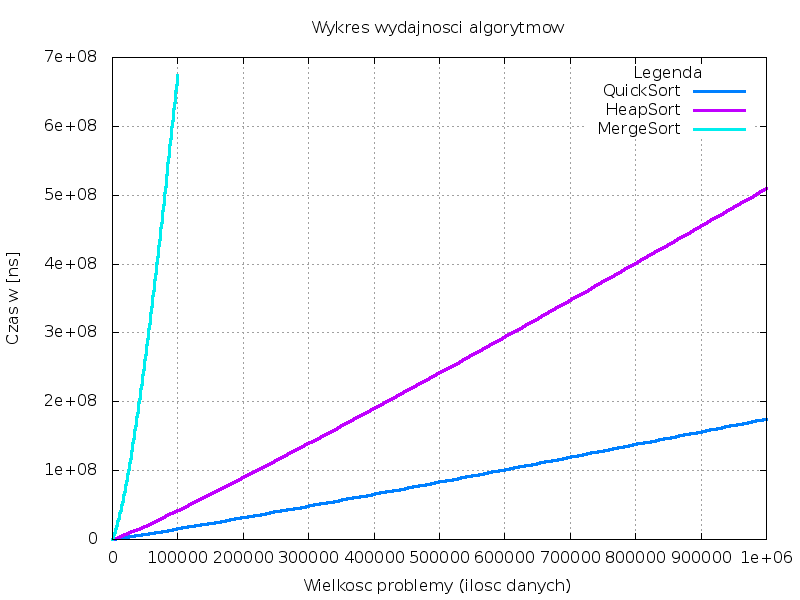
\includegraphics[scale = 0.4]{Eksperyment.png}
	\end{figure}
\end{center}


\section{Wnioski}
Uzyskane przeze mnie wyniki jednoznacznie określają, iż najlepiej z problemem poradził sobie algorytm szybkiego sortowania. Jest on najwydajniejszym algorytmem, mimo
że w pewnych sytuacjach jego złożoność obliczeniowa może być nawet kwadratowa. Algorytm ten jest często stosowany w informatyce dzięki swojej szybkości. Drugi pod
względem szybkości był algorytm sortowania kopcowego. Uważam, że algorytm ten działał dłużej ze względu na potrzebę przeorganizowania całej tablicy danych, a także
porządkowanie i naprawę kopca. W przypadku QuickSorta wynkonywane jest praktycznie tylko dzielenie i rekurencyjne wywołanie. Zadałem więc sobie pytanie, dlaczego
w klasie algorytmów o wydajności (n ln n) to właśnie algorytm sortowania przez scalanie okazał się najwolniejszy, wszak podobnie jak QuickSort bazuje na zasadzie:
dziel i zwyciężaj, i również opiera się na podziale tablicy. Doszedłem do wniosku, że przewagą QuickSortu jest pre-sortowanie, w postaci umieszczania elementów
większych od pewnego znacznika w jednej tablicy i mniejszych w drugiej. Dzięki temu jedyną pozostałą po posortowaniu sub-tablic operacją jest ich połączenie, a w
przypadku MergeSort'a dodatkowo musimy jeszcze posortować pomniejsze tablice i dopiero złączyć je, z tych pojedyńczyć klocków, w całość.
\end{document}
